\chapter{Data warehouse}


\begin{description}
    \item[\Acl{bi}] \marginnote{\Acl{bi}}
        Transform raw data into information.
        Deliver the right information to the right people at the right time through the right channel.

    \item[\Ac{dwh}] \marginnote{\Acl{dwh}}
        Optimized repository that stores information for decision-making processes.
        \Acp{dwh} are a specific type of \ac{dss}.

        Features:
        \begin{itemize}
            \item Subject-oriented: focused on enterprise-specific concepts.
            \item Integrates data from different sources and provides a unified view.
            \item Non-volatile storage with change tracking. 
        \end{itemize}

    \item[\Ac{dm}] \marginnote{\Acl{dm}}
        Subset of the primary \ac{dwh} with information relevant to a specific business area.
\end{description}



\section{\Acl{olap} (\Acs{olap})}

\begin{description}
    \item[\ac{olap} analyses] \marginnote{\Acl{olap} (\Acs{olap})}
        Able to interactively navigate the information in a data warehouse.
        Allows to visualize different levels of aggregation.

    \item[\ac{olap} session] 
        Navigation path created by the operations that a user applied.
\end{description}

\begin{figure}[H]
    \centering
    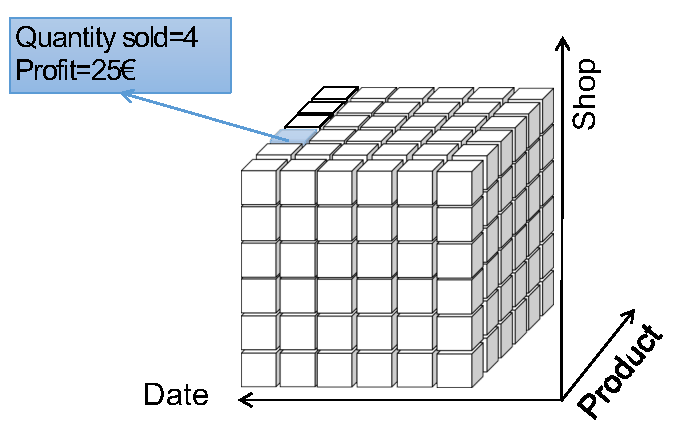
\includegraphics[width=0.35\textwidth]{img/_olap_cube.pdf}
    \caption{\ac{olap} data cube}
\end{figure}


\subsection{Operators}

\begin{description}
    \item[Roll-up] \marginnote{Roll-up}
        \begin{minipage}{0.7\textwidth}
            Increases the level of aggregation (i.e. \texttt{GROUP BY} in SQL).
            Some details are collapsed together.
        \end{minipage}
        \hfill
        \begin{minipage}{0.15\textwidth}
            \centering
            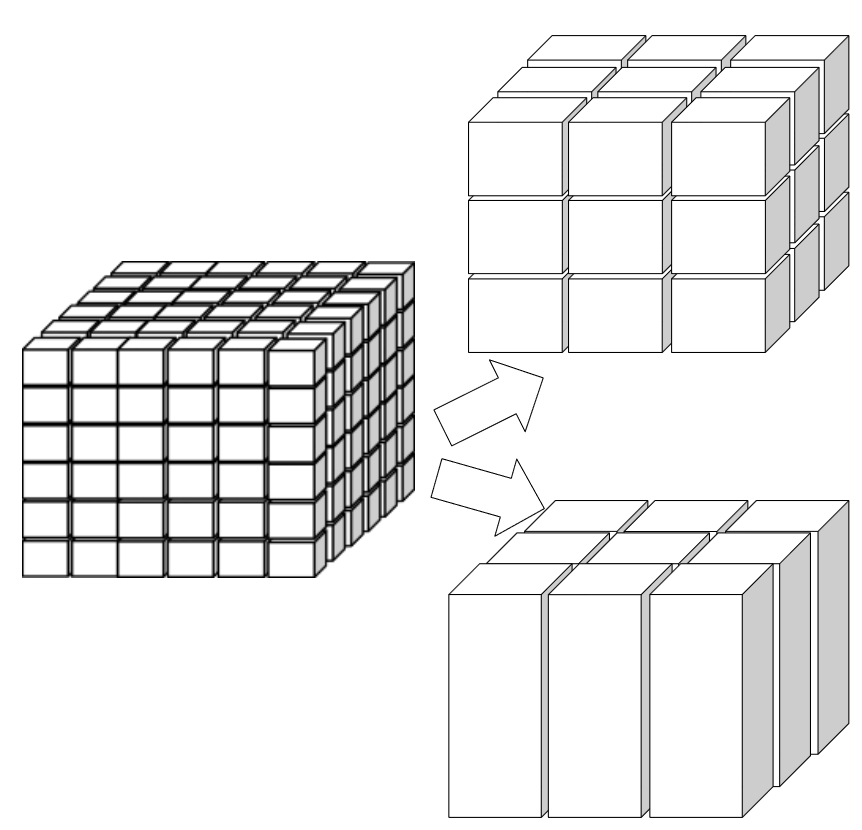
\includegraphics[width=\linewidth]{img/olap_rollup.png}
        \end{minipage}

    \item[Drill-down] \marginnote{Drill-down}
        \begin{minipage}{0.7\textwidth}
            Reduces the level of aggregation.
            Some details are reintroduced.
        \end{minipage}
        \hfill
        \begin{minipage}{0.15\textwidth}
            \centering
            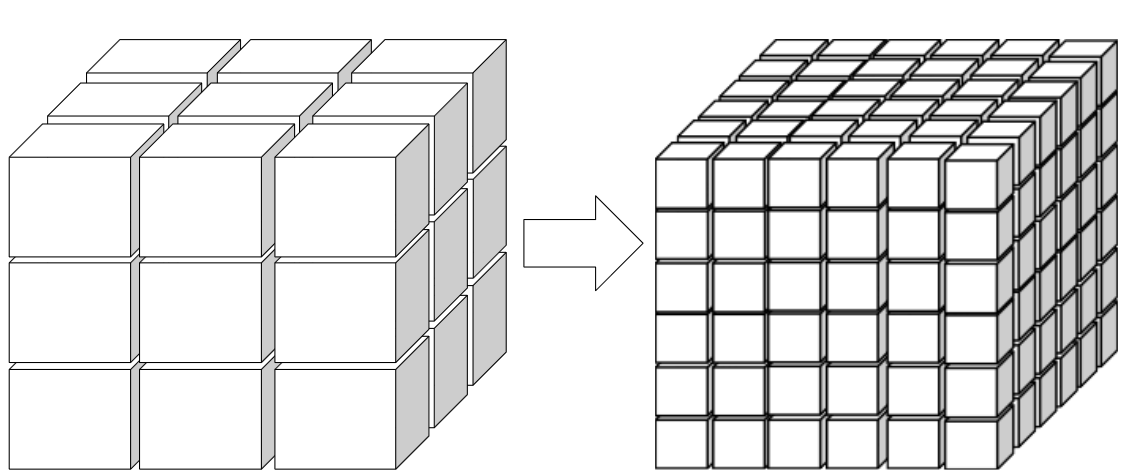
\includegraphics[width=\linewidth]{img/olap_drilldown.png}
        \end{minipage}
    
    \item[Slide-and-dice] \marginnote{Slide-and-dice}
        \begin{minipage}{0.65\textwidth}
            The slice operator reduces the number of dimensions (i.e. drops columns).

            The dice operator reduces the number of data being analyzed (i.e. \texttt{LIMIT} in SQL).
        \end{minipage}
        \hfill
        \begin{minipage}{0.15\textwidth}
            \centering
            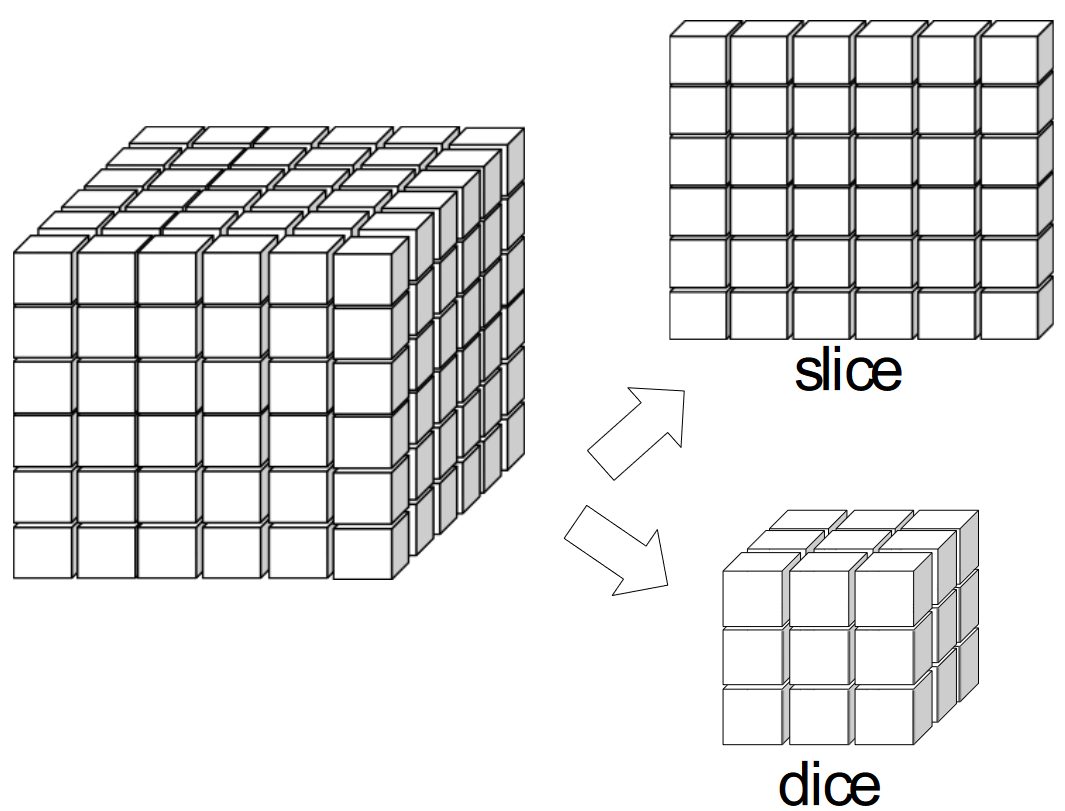
\includegraphics[width=\linewidth]{img/olap_slicedice.png}
        \end{minipage}    

    \item[Pivot] \marginnote{Pivot}
        \begin{minipage}{0.7\textwidth}
            Changes the layout of the data, to analyze it from a different viewpoint.
        \end{minipage}
        \hfill
        \begin{minipage}{0.15\textwidth}
            \centering
            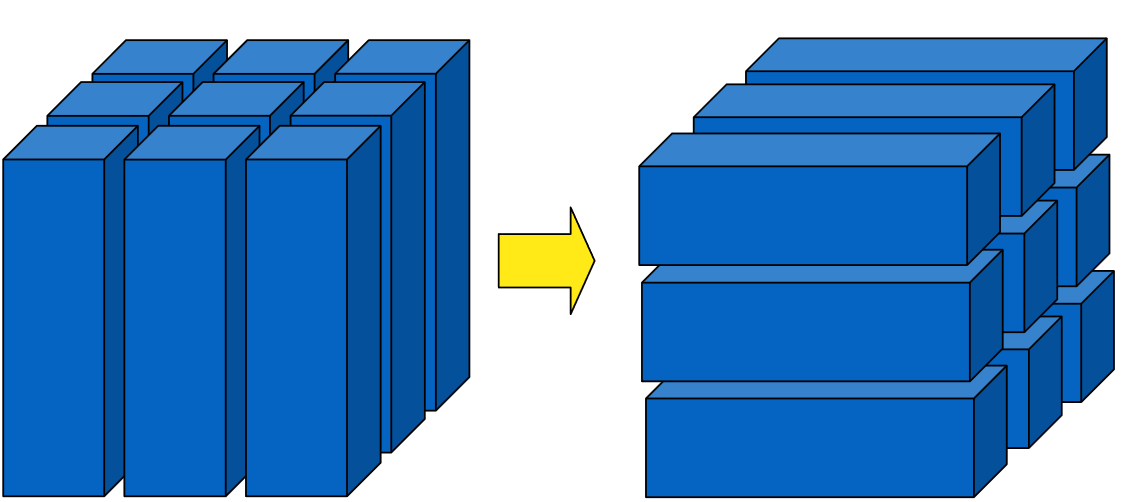
\includegraphics[width=\linewidth]{img/olap_pivot.png}
        \end{minipage}

    \item[Drill-across] \marginnote{Drill-across}
        \begin{minipage}{0.7\textwidth}
            Links concepts from different data sources (i.e. \texttt{JOIN} in SQL).
        \end{minipage}
        \hfill
        \begin{minipage}{0.15\textwidth}
            \centering
            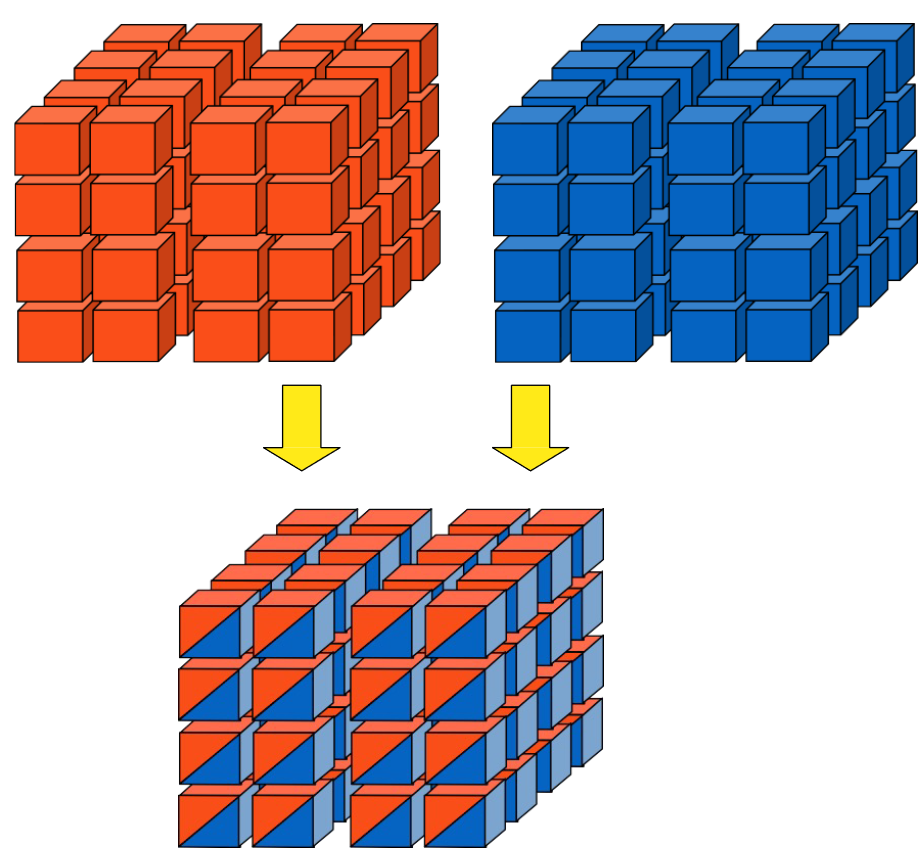
\includegraphics[width=\linewidth]{img/olap_drillacross.png}
        \end{minipage}    
    
    \item[Drill-through] \marginnote{Drill-through}
        Switches from multidimensional aggregated data to operational data (e.g. a spreadsheet).
        \begin{center}
            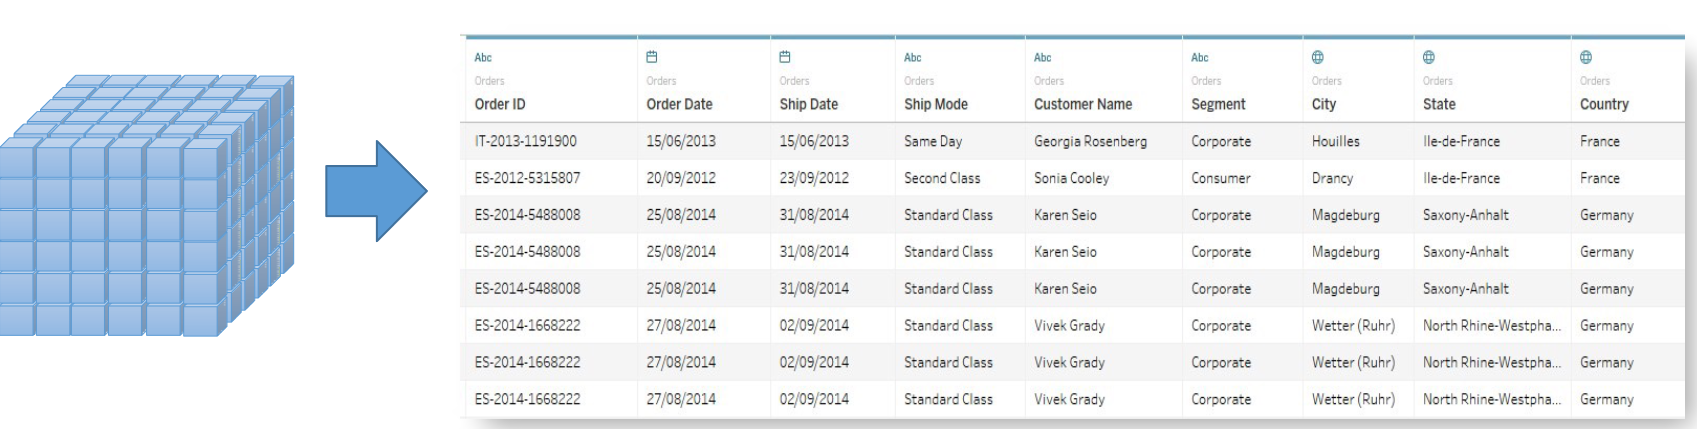
\includegraphics[width=0.5\textwidth]{img/olap_drillthrough.png}
        \end{center}    
\end{description}



\section{\Acl{etl} (\Acs{etl})}
\marginnote{\Acl{etl} (\Acs{etl})}
The \Ac{etl} process extracts, integrates and cleans operational data that will be loaded into a data warehouse.


\subsection{Extraction}

Extracted operational data can be:
\begin{descriptionlist}
    \item[Structured] \marginnote{Strucured data}
        with a predefined data model (e.g. relational DB, CSV)

    \item[Untructured] \marginnote{Unstrucured data}
        without a predefined data model (e.g. social media content)
\end{descriptionlist}

Extraction can be of two types:
\begin{descriptionlist}
    \item[Static] \marginnote{Static extraction}
        The entirety of the operational data are extracted to populate the
        data warehouse for the first time.
    
    \item[Incremental] \marginnote{Incremental extraction}
        Only changes applied since the last extraction are considered.
        Can be based on a timestamp or a trigger.
\end{descriptionlist}


\subsection{Cleaning}

Operational data may contain:
\begin{descriptionlist}
    \item[Duplicate data] 
    \item[Missing data] 
    \item[Improper use of fields] (e.g. saving the phone number in the \texttt{notes} field)
    \item[Wrong values] (e.g. 30th of February)
    \item[Inconsistencies] (e.g. use of different abbreviations)
    \item[Typos]    
\end{descriptionlist}

Methods to clean and increase the quality of the data are:
\begin{descriptionlist}
    \item[Dictionary-based techniques] \marginnote{Dictionary-based cleaning}
        Lookup tables to substitute abbreviations, synonyms or typos.
        Applicable if the domain is known and limited.
        
    \item[Approximate merging] \marginnote{Approximate merging}
        Methods to merge data that do not have a common key.
        \begin{description}
            \item[Approximate join]
                Use non-key attributes to join two tables (e.g. using the name and surname instead of a unique identifier).

            \item[Similarity approach]
                Use similarity functions (e.g. edit distance) to merge multiple instances of the same information
                (e.g. typo in customer surname).
        \end{description}
    
    \item[Ad-hoc algorithms] \marginnote{Ad-hoc algorithms}
\end{descriptionlist}


\subsection{Transformation}
Data are transformed to respect the format of the data warehouse:
\begin{descriptionlist}
    \item[Conversion] \marginnote{Conversion}
        Modifications of types and formats (e.g. date format)
    
    \item[Enrichment] \marginnote{Enrichment}
        Creating new information by using existing attributes (e.g. compute profit from receipts and expenses)

    \item[Separation and concatenation] \marginnote{Separation and concatenation}
        Denormalization of the data: introduces redundancies (i.e. breaks normal form\footnote{\url{https://en.wikipedia.org/wiki/Database_normalization}}) 
        to speed up operations.
\end{descriptionlist}


\subsection{Loading}
Adding data into a data warehouse:
\begin{descriptionlist}
    \item[Refresh] \marginnote{Refresh loading}
        The entire \ac{dwh} is rewritten.

    \item[Update] \marginnote{Update loading}
        Only the changes are added to the \ac{dwh}. Old data are not modified.
\end{descriptionlist}



\section{Data warehouse architectures}

The architecture of a data warehouse should meet the following requirements:
\begin{descriptionlist}
    \item[Separation] Separate the analytical and transactional workflows.
    \item[Scalability] Hardware and software should be easily upgradable.
    \item[Extensibility] Capability to host new applications and technologies without the need to redesign the system.
    \item[Security] Access control.
    \item[Administrability] Easily manageable.
\end{descriptionlist}

\subsection{Single-layer architecture}
\marginnote{Single-layer architecture}
\begin{minipage}{0.55\textwidth}
    \begin{itemize}
        \item Minimizes the amount of data stored (i.e. no redundances).
        \item The source layer is the only physical layer (i.e. no separation).
        \item A middleware provides the \ac{dwh} features.
    \end{itemize}
\end{minipage}
\hfill
\begin{minipage}{0.4\textwidth}
    \centering
    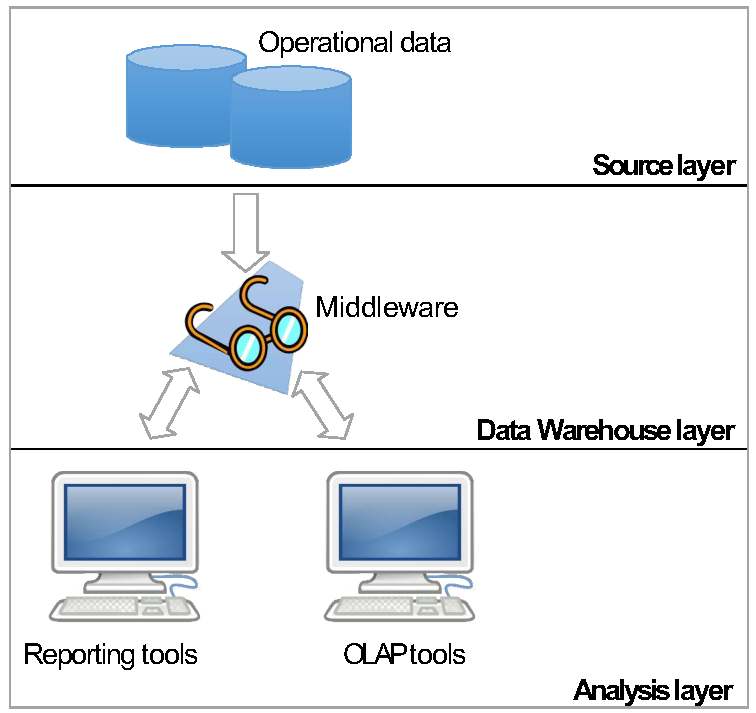
\includegraphics[width=\linewidth]{img/_1layer_dwh.pdf}
\end{minipage}


\subsection{Two-layer architecture}
\marginnote{Two-layer architecture}
\begin{minipage}{0.55\textwidth}
    \begin{itemize}
        \item Source data (source layer) are physically separated from the \ac{dwh} (data warehouse layer).
        \item A staging layer applies \ac{etl} procedures before populating the \ac{dwh}.
        \item The \ac{dwh} is a centralized repository from which data marts can be created.
            Metadata repositories store information on sources, staging and data marts schematics.
    \end{itemize}
\end{minipage}
\hfill
\begin{minipage}{0.4\textwidth}
    \centering
    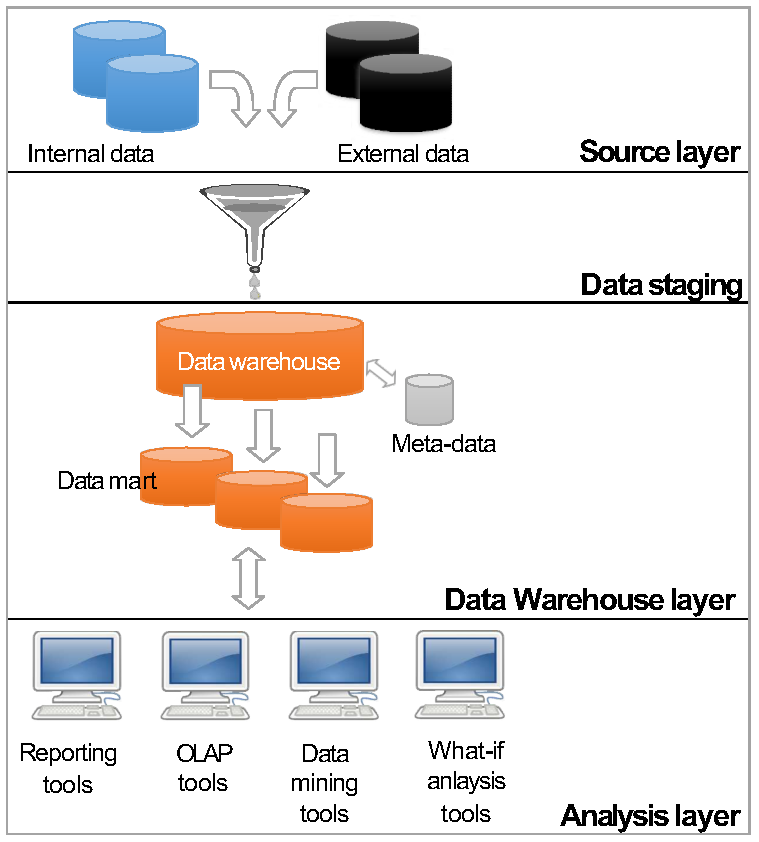
\includegraphics[width=\linewidth]{img/_2layer_dwh.pdf}
\end{minipage}


\subsection{Three-layer architecture}
\marginnote{Three-layer architecture}
\begin{minipage}{0.45\textwidth}
    \begin{itemize}
        \item A reconciled layer enhances the cleaned data coming from the staging step by 
            adding enterprise-level details (i.e. adds more redundancy before populating the \ac{dwh}).
    \end{itemize}
\end{minipage}
\hfill
\begin{minipage}{0.5\textwidth}
    \centering
    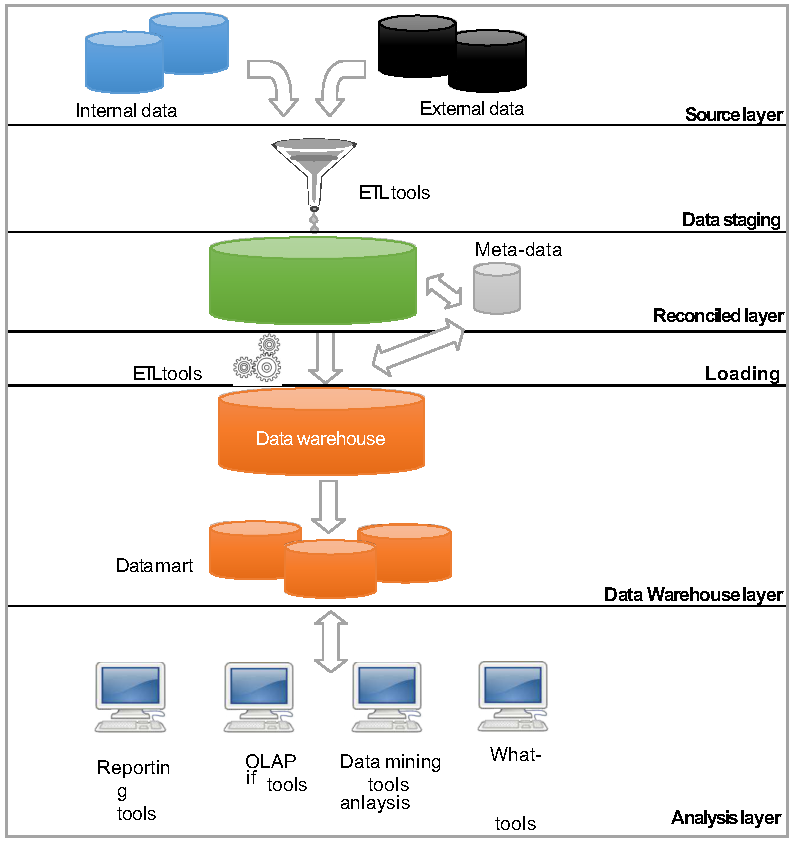
\includegraphics[width=\linewidth]{img/_3layer_dwh.pdf}
\end{minipage}



\section{Conceptual modeling}

\begin{description}
    \item[\Acl{dfm} (\acs{dfm})] \marginnote{\Acl{dfm} (\acs{dfm})}
        Conceptual model to support the design of data marts.
        The main concepts are:
        \begin{descriptionlist}
            \item[Fact] 
                Concept relevant to decision-making processes (e.g. sales).
            \item[Measure]
                Numerical property to describe a fact (e.g. profit).
            \item[Dimension] 
                Property of a fact with a finite domain (e.g. date).
            \item[Dimensional attribute] 
                Property of a dimension (e.g. month).
            \item[Hierarchy] 
                A tree where the root is a dimension and nodes are dimensional attributes (e.g. date $\rightarrow$ month).
            \item[Primary event] 
                Occurrence of a fact. It is described by a tuple with a value for each dimension and each measure.
            \item[Secondary event] 
                Aggregation of primary events. 
                Measures of primary events are aggregated if they have the same (preselected) dimensional attributes.
        \end{descriptionlist}
\end{description}

\begin{figure}[H]
    \centering
    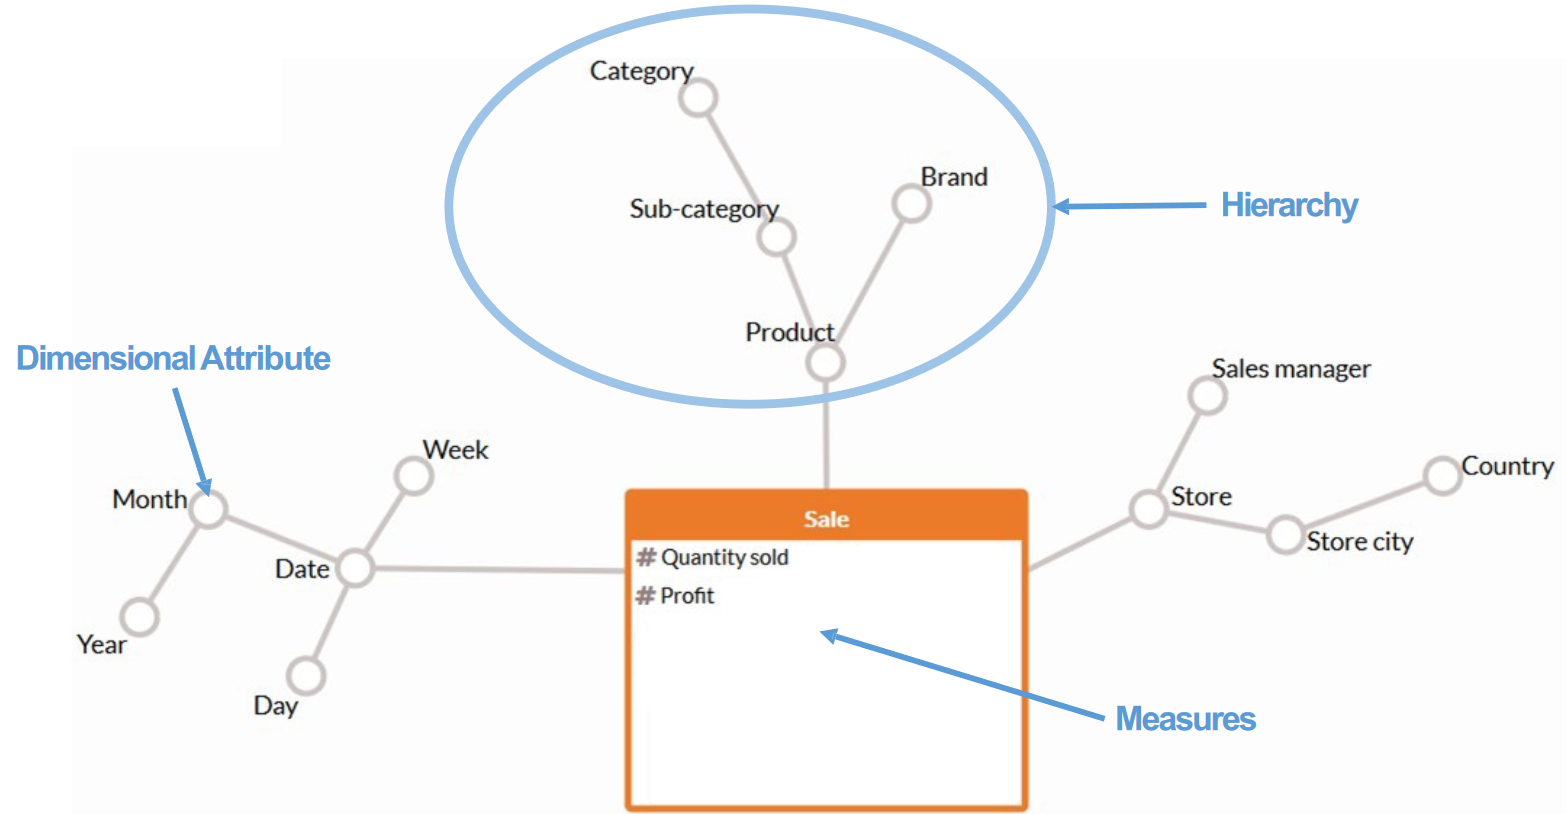
\includegraphics[width=0.8\textwidth]{img/dfm.png}
    \caption{Example of \ac{dfm}}
\end{figure}

\begin{figure}[H]
    \centering
    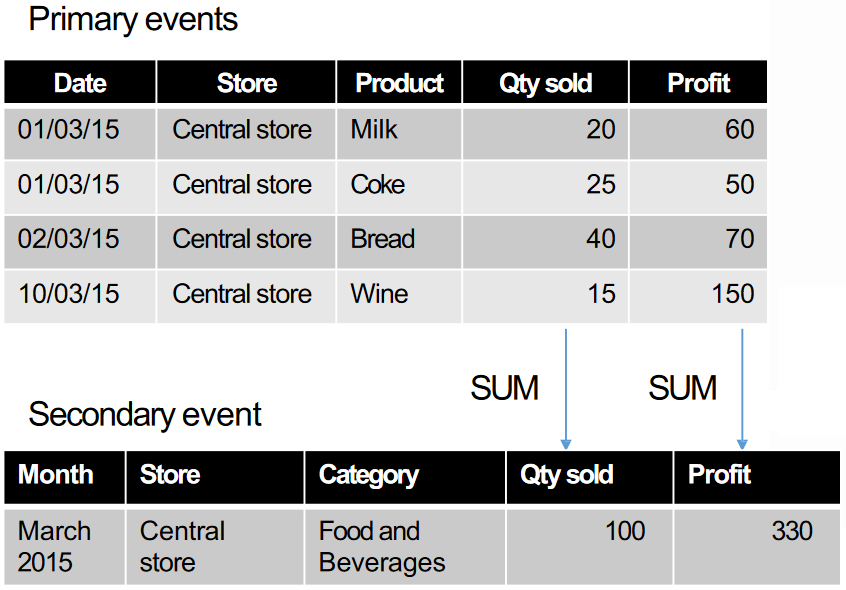
\includegraphics[width=0.5\textwidth]{img/dfm_events.png}
    \caption{Example of primary and secondary events}
\end{figure}


\subsection{Aggregation operators}

Measures can be classified as:
\begin{descriptionlist}
    \item[Flow measures] \marginnote{Flow measures}
        Evaluated cumulatively with respect to a time interval (e.g. quantity sold).
    \item[Level measures] \marginnote{Level measures}
        Evaluated at a particular time (e.g. number of products in inventory).
    \item[Unit measures] \marginnote{Unit measures}
        Evaluated at a particular time but expressed in relative terms (e.g. unit price).
\end{descriptionlist}

Aggregation operators can be classified as:
\begin{descriptionlist}
    \item[Distributive] \marginnote{Distributive operators}
        Able to calculate aggregates from partial aggregates (e.g. \texttt{SUM}, \texttt{MIN}, \texttt{MAX}).
    \item[Algebraic] \marginnote{Algebraic operators}
        Requires a finite number of support measures to compute the result (e.g. \texttt{AVG}).
    \item[Holistic] \marginnote{Holistic operators}
        Requires an infinite number of support measures to compute the result (e.g. \texttt{RANK}).
\end{descriptionlist}

\begin{description}
    \item[Additivity] \marginnote{Additive measure}
    A measure is additive along a dimension if an aggregation operator can be applied. 
    \begin{table}[H]
        \centering
        \begin{tabular}{l | c | c}
                                        & \textbf{Temporal hierarchies}                             & \textbf{Non-temporal hierarchies} \\
            \hline
            \textbf{Flow measures}      & \texttt{SUM}, \texttt{AVG}, \texttt{MIN}, \texttt{MAX}    & \texttt{SUM}, \texttt{AVG}, \texttt{MIN}, \texttt{MAX} \\
            \textbf{Level measures}     & \texttt{AVG}, \texttt{MIN}, \texttt{MAX}                  & \texttt{SUM}, \texttt{AVG}, \texttt{MIN}, \texttt{MAX} \\
            \textbf{Unit measures}      & \texttt{AVG}, \texttt{MIN}, \texttt{MAX}                  & \texttt{AVG}, \texttt{MIN}, \texttt{MAX} \\
        \end{tabular}
        \caption{Allowed operators for each measure type}
    \end{table}
\end{description}



\section{Logical design}
\marginnote{Logical design}
Defining the data structures (e.g. tables and relationships) according to a conceptual model.
There are two main strategies:
\begin{descriptionlist}
    \item[Star schema] \marginnote{Star schema}
        A fact table that contains all the measures is linked to dimensional tables.
        \begin{figure}[H]
            \centering
            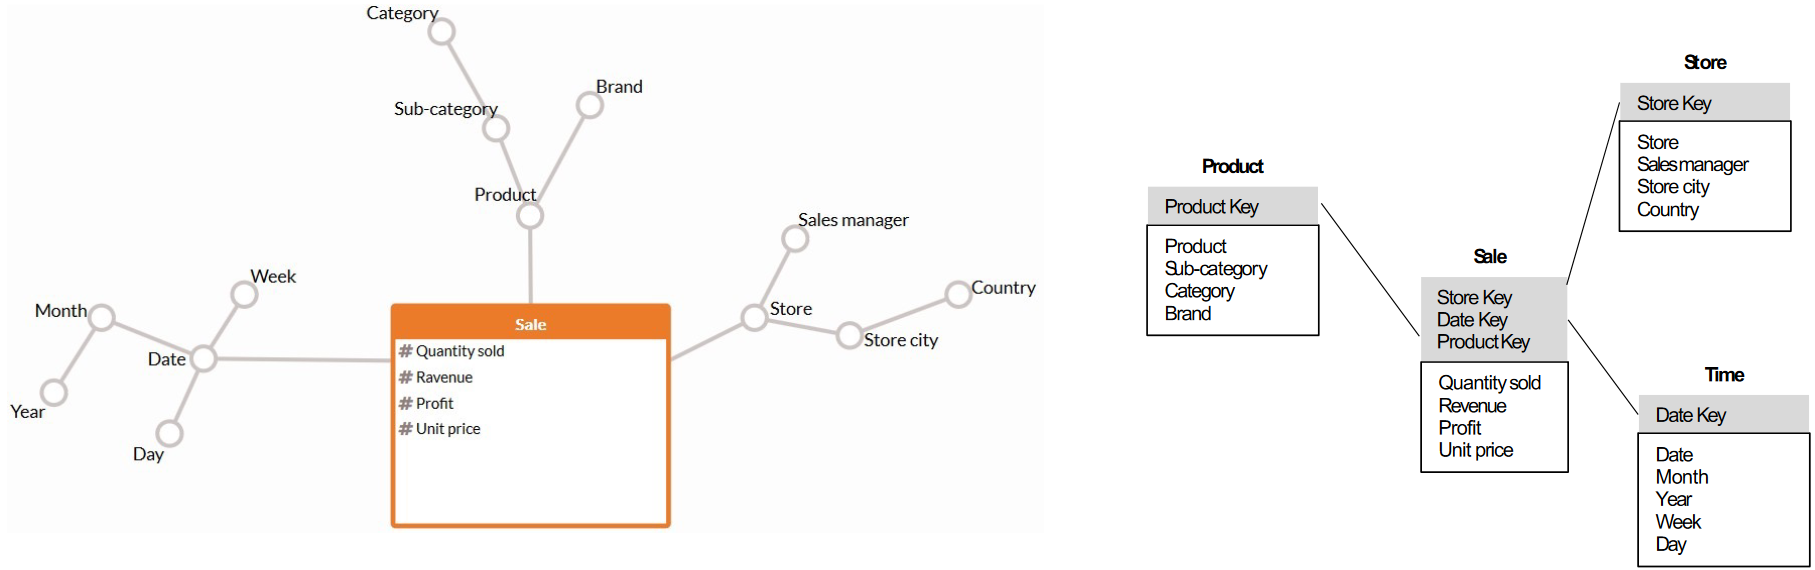
\includegraphics[width=\textwidth]{img/logical_star_schema.png}
            \caption{Example of star schema}
        \end{figure}

    \item[Snowflake schema] \marginnote{Snowflake schema}
        A star schema variant with partially normalized dimensional tables.
        \begin{figure}[H]
            \centering
            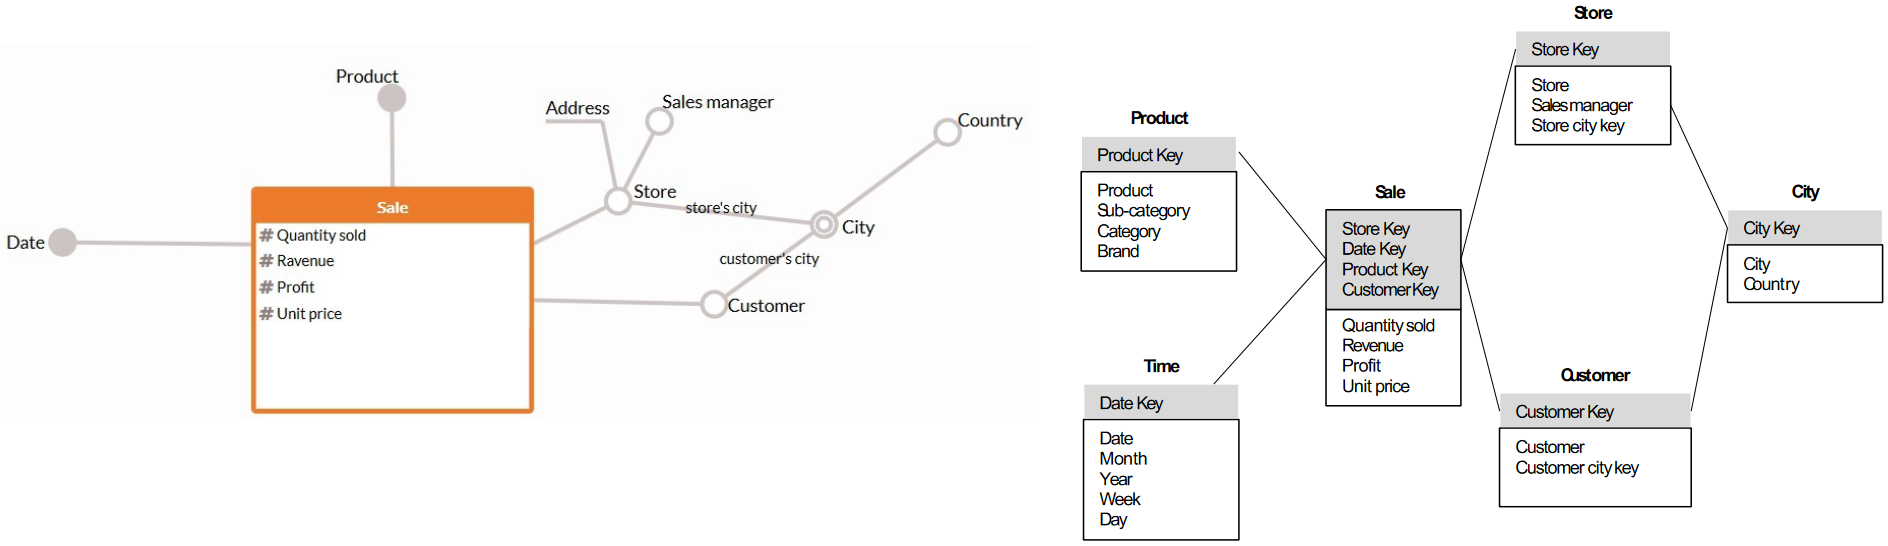
\includegraphics[width=\textwidth]{img/logical_snowflake_schema.png}
            \caption{Example of snowflake schema}
        \end{figure}
\end{descriptionlist}